% File clic2021.tex
% May 2021

%% Based on the style files for CLiC-IT-2019, which were, in turn,
%% Based on the style files for CLiC-IT-2014, which were, in turn,
%% Based on the style files for ACL-2014, which were, in turn,
%% Based on the style files for ACL-2013, which were, in turn,
%% Based on the style files for ACL-2012, which were, in turn,
%% based on the style files for ACL-2011, which were, in turn,
%% based on the style files for ACL-2010, which were, in turn,
%% based on the style files for ACL-IJCNLP-2009, which were, in turn,
%% based on the style files for EACL-2009 and IJCNLP-2008...
%% Based on the style files for EACL 2006 by
%% e.agirre@ehu.es or Sergi.Balari@uab.es
%% and that of ACL 08 by Joakim Nivre and Noah Smith

\documentclass[11pt]{article}
\usepackage[a4paper]{geometry}
\usepackage{clic2023} % imports CLiC-it 2023 layout style
\usepackage{times} % font
\usepackage{xurl} % splits URL in multiple lines
\usepackage[italian,english]{babel}
\usepackage{latexsym}
\pagenumbering{gobble} % does not display page numbering
\usepackage{xcolor}
\usepackage{multirow}
\usepackage{todonotes}
\usepackage{subcaption}
\usepackage{amssymb}
\usepackage{float}
\usepackage{cuted}
\usepackage{soul}
\usepackage{xcolor}
\usepackage{ulem}

\definecolor{lightgreen}{RGB}{0, 180, 0}
\definecolor{lightred}{RGB}{214, 0, 0}

\newcommand{\hlg}[1]{{\sethlcolor{lightgreen}\hl{#1}}}
\newcommand{\hlr}[1]{{\sethlcolor{lightred}\hl{#1}}}


\newcommand{\bs}[0]{$\blacksquare$}

\newcommand{\Ni}{({\em i})~}
\newcommand{\Nii}{({\em ii})~}
\newcommand{\Niii}{({\em iii})~}

\newcommand{\abc}[1]{{\color{blue} #1}}
\newcommand{\paolo}[1]{{\color{red} #1}}

\newcommand{\todoA}[1]{\todo[color=blue!40]{A: #1}}
\newcommand{\todoP}[1]{\todo[color=red]{P: #1}}

\newcommand{\itodo}[1]{\todo[inline]{#1}}

\newcommand{\dsENcorpus}{IFU-22-EN}
\newcommand{\dsITcorpus}{IFU-22-IT}
\newcommand{\dsENclassification}{IFS-EN}
\newcommand{\dsITclassification}{IFS-IT}
\newcommand{\dsENforecasting}{IFSS-EN-223K}
\newcommand{\dsITforecasting}{IFSS-IT-30K}

\newcommand{\bert}{\mbox{BERT$_{base}$}}
\newcommand{\mbert}{\mbox{mBERT$_{base}$}}
\newcommand{\imbert}{\mbox{Incel mBERT}}
\newcommand{\umbert}{\mbox{UmBERTo}}
\newcommand{\albert}{\mbox{AlBERTo}}
\newcommand{\iumbert}{\mbox{Incel UmBERTo}}
\newcommand{\ialbert}{\mbox{Incel AlBERTo}}

\newcommand{\hsdfb}{\mbox{HSD-FB}}
\newcommand{\hsdtw}{\mbox{HSD-TW}}
\newcommand{\ami}{\mbox{AMI-20}}


\newcommand{\dsENclassificationtrain}{IFS-EN$_{\mbox{tr}}$} % Incel Forum Supervised, English, 5203 instances
\newcommand{\dsENclassificationdev}{IFS-EN$_{\mbox{de}}$} % Incel Forum Supervised, English, 5203 instances
\newcommand{\dsENclassificationtest}{IFS-EN$_{\mbox{te}}$} % Incel Forum Supervised, English, 5203 instances

\newcommand{\enforum}{\textit{Incels.is}}
\newcommand{\itforum}{\textit{Il forum dei brutti}}

%\setlength\titlebox{5cm}

% You can expand the titlebox if you need extra space
% to show all the authors. Please do not make the titlebox
% smaller than 5cm (the original size); we will check this
% in the camera-ready version and ask you to change it back.


  \title{Hate Speech Detection in an Italian Incel Forum \\ Using Bilingual Data for Pre-Training and Fine-Tuning}

\author{\textbf{Paolo Gajo, Silvia Bernardini, Adriano Ferraresi and Alberto Barr\'on-Cede\~no} \\
  DIT, Universit\`a di Bologna, Forl\`i, Italy \\
  {\tt paolo.gajo@studio.unibo.it}\\
  {\tt \{silvia.bernardini, adriano.ferraresi, a.barron\}@unibo.it}}

\date{}

\begin{document}
\maketitle
\begin{abstract}
  % \todo{I changed the first instance. You are not doing it on the forum, but on a corpus you download from that forum. Please change the Italian verison accordingly}
\textbf{English.}~In this study, we aim to enhance hate speech detection in Italian incel posts.
% , short for ``involuntary celibates''
We pre-train monolingual (Italian) and multilingual Transformer models on corpora built from two incel forums, one in Italian and one in English, using masked language modeling. Then, we fine-tune the models on combinations of English and Italian corpora, annotated for hate speech.
% , built from incel forums and mainstream social media sites.
% with binary labels which indicate whether a post contains hate speech or not. The Italian training datasets are compiled from mainstream social media (Twitter and Facebook), while the English dataset is built by gathering posts from the English incel forum. The models' performance is evaluated on the Italian incel forum dataset.
Experiments on a hate speech corpus derived from the Italian incel forum show that the best results are achieved by training multilingual models on bilingual data,
rather than training monolingual models on Italian-only data. This emphasizes the importance of using training and testing data from a similar linguistic domain, even when the languages differ.

% HS identification in cross-lingual and cross-domain settings. We do so by employing Transformer models, pre-trained on monolingual (Italian) and bilingual (Italian-English) corpora. We fine-tune these models on various combinations of English- and Italian-language datasets, all annotated for HS. The English-language dataset pertains to the so-called community of ``incels'', short for ``involuntary celibates'', while the ones in Italian are compiled from mainstream social media sites (Twitter and Facebook). We then evaluate the performance of the models on an Italian-language dataset built from the contents of an Italian incel forum. Our experiments with model domain adaptation via training on the masked language modeling task and fine-tuning on different combinations of datasets show that the best results are obtained not by training solely using Italian data, but with a combination of Italian and English data. This shows the importance of using in-domain data for training, even when training and test data are in different languages.

\end{abstract}

\begin{abstract-alt}
  % \todoA{change Italian according to en modifs}
\textrm{\bf{Italiano.}}~In questo studio, ci proponiamo di migliorare il rilevamento dei discorsi d'odio in post tratti da un forum italiano di incel.
%  , abbreviazione di ``celibi involontari''.
Addestriamo modelli Transformer mono (italiano) e multilingue su corpora ottenuti da due forum di incel, uno in italiano e uno in inglese, con il masked language modeling. Facciamo quindi il fine-tuning dei modelli su corpora in italiano e inglese con annotazioni indicanti se un post esprime odio.
%  , costruiti a partire da social media di vasto utilizzo e forum di incel.
Sperimentando su un corpus annotato per i discorsi di odio ottenuto da un forum italiano di incel mostriamo che i risultati migliori si ottengono addestrando modelli multilingue su combinazioni bilingue di corpora e non con modelli italiani e dati monolingue. Ciò sottolinea l'importanza di utilizzare dati di addestramento appartenenti a un contesto linguistico simile a quello dei dati di valutazione, anche con lingue differenti.
%  di addestramento e valutazione

%  . A questo scopo, impieghiamo modelli Transformer, pre-addestrati su corpora monolingui (italiano) e bilingui (italiano-inglese). Abbiamo effettuato il fine-tuning di questi modelli su varie combinazioni di dataset in lingua inglese e italiana, tutti annotati per i discorsi d'odio. Il dataset inglese riguarda la comunità dei c.d. ``incel'', abbreviazione inglese di ``celibi involontari'', mentre quelli italiani sono costruiti partendo da social media di vasto utilizzo (Twitter e Facebook). Valutiamo le prestazioni dei modelli su un dataset in lingua italiana costruito a partire dai contenuti di un forum italiano di incel. Gli esperimenti di adattamento dei modelli a questo contesto linguistico attraverso l'addestramento sulla task del masked language modeling e il fine-tuning su diverse combinazioni di dataset dimostrano che i risultati migliori si ottengono non solo con l'addestramento su dati in italiano, ma con una combinazione di dati in italiano e in inglese. Questo dimostra l'importanza di utilizzare dati provenienti dallo stesso contesto linguistico per l'addestramento, anche quando i dati di addestramento e di test sono in lingue diverse.
\end{abstract-alt}


\section{Introduction}

% Hate speech, broadly defined as language that expresses hatred towards a targeted group or is intended to be derogatory, humiliating, or insulting to the members of the group~\cite{davidson-2017-automated-hate}, has become an increasingly prevalent and dangerous phenomenon~\cite{matamoros-fernandezRacismHateSpeech2021}.
% % The rapid rise of social media platforms has enabled the dissemination of hateful and offensive rhetoric, with tangible negative consequences, such as increased prejudice towards minority groups and the escalation of hate crimes \cite{peliconInvestigatingCrosslingualTraining2021}.
%  A specific area of concern in the realm of hate speech is the online spaces known as the ``Manosphere'', where misogynous discourse in particular has become increasingly rampant~\cite{ribeiro2021evolution-manosphere}.
% % These spaces are characterized by the adoption of the ``Red Pill'' philosophy, which promotes a toxic idea of masculinity and traditional gender roles, and has been linked to the rise in misogynous and racist discourse~\cite{gingAlphasBetasIncels2019-manosphere}.
% Specifically, within the Manosphere, the incel (short for ``involuntary celibate'') community has been identified as frequently engaging in hateful, misogynous, and racist speech~\cite{nagle-2017-kill-normies,jakiOnlineHatredWomen2019}.
% Given the gravity of the phenomenon, especially in these environments, the development of effective hate speech detection systems is critical to addressing the harmful consequences of these online platforms and promoting a more inclusive and respectful digital landscape.

While there is no scarcity of English-language models and training resources for
the detection of hate speech (HS), especially with the recent rise in popularity of
this research topic~\cite{alkomahLiteratureReviewTextual2022},
much work can still be done when approaching this problem in other languages.
For less-resourced languages, such as Italian, one of the main difficulties of combating this phenomenon is the lack of annotated data~\cite{van2023mitigating}. The problem becomes even more
exacerbated when considering the detection of hate speech in niche contexts,
such as in forums frequented by incels,
short for ``involuntary celibates'', a community known for its hateful language \cite{nagle-2017-kill-normies,jakiOnlineHatredWomen2019}
and use of
specific misogynous and racist lexicon \cite{farrellExploringMisogynyManosphere2019,gothard2020exploring}.
In particular, it seems no work has yet been done on the detection of hate speech in Italian incel forums.

In this paper, we present a simple approach to improve the performance of hate speech detection models in Italian forums frequented by incels. Our contribution is two-fold:

% \paragraph{\Ni Corpora} We compile two novel unsupervised corpora on the domain of incel forums, one in Italian and one in English. We annotate a subset of each for hate speech, misogyny, and racism, obtaining two supervised corpora. The unsupervised corpora can be used for domain-adaptation, while the supervised ones can be used for training hate speech detection models.

\noindent\textbf{\Ni Masked language modeling.} We adapt monolingual Italian models and a multilingual model to the linguistic domain of Italian and English incel forums by training them on the masked language modeling (MLM) task.
As training material, we use unsupervised corpora built from two incel forums, one in Italian and one in English.
We release these novel models, which can be used for further research on the topic.\footnote{Links to the models, released on HuggingFace: \url{https://github.com/paolo-gajo/clic23}.} 

\noindent\textbf{\Nii Hate speech detection.}
% \todoA{experiments are not contributions. You should stress the outcome more. I see you have a paragraph on it next, perhaps merge}
We fine-tune the vanilla and domain-adapted models on the downstream task of detecting hate speech in Italian incel posts. %forums.
% We do this by fine-tuning them on combinations of Italian and English-language supervised corpora.
% The corpora were compiled from incel forums and mainstream social media platforms and are binary-annotated for hate speech.
Monolingual models are trained on Italian-only combinations of corpora binary-annotated for hate speech, while Italian--English combinations are used for the multilingual models.

Testing the performance of the models on a labelled hate speech corpus, obtained by annotating posts from the Italian incel forum, shows that the best results are obtained by first training the base multilingual model on bilingual data taken from both the Italian and English incel forums, using the MLM task, and then fine-tuning it on combinations of Italian and English corpora, annotated for hate speech. In the approached scenarios, pre-training and fine-tuning on bilingual in-domain incel annotated data may therefore be more effective than training on general target-language supervised corpora, despite part of the training data not being in the language of the downstream task. In addition, the results show that this strategy can be used to improve model performance when in-domain target-language data is scarce, by using in-domain data from other languages.

The rest of the paper is organized as follows: Section~\ref{sec:related-work} presents related work on hate speech detection in Italian and English, as well as multilingual approaches to the problem. Section~\ref{sec:corpora} describes the corpora used in this study. Section~\ref{sec:models} presents the employed models. Section~\ref{sec:exps} describes the experiments conducted and discusses the results. Section~\ref{sec:conclusions} closes the contribution with conclusions and future work.
% \vspace*{1mm}

% To this end, we train Transformer models on a variety of datasets in English and Italian, all annotated for hate speech. The English training dataset is compiled from an English-language incel forum, \enforum\footnote{\url{https://incels.is}}, while the Italian ones are built from mainstream social media platforms such as Twitter and Facebook.

% We use two mBERT~\cite{devlinBERTPretrainingDeep2019a} models as the baselines for our study, training them on both the English and the Italian datasets. We compare \mbert\, to another mBERT model, trained on the masked language modeling (MLM) task on sentences extracted from two incel forums, one in English (\enforum) and one in Italian (\itforum\footnote{\url{https://ilforumdeibrutti.forumfree.it}}).
% The two mBERT models are compared to other models trained specifically on Italian data: \umbert\, \cite{musixmatch-2020-umberto} and \albert\, \cite{PolignanoEtAlCLIC2019}. We also train these two models on the MLM task on the entirety of the contents of the aforementioned Italian incel forum. In doing so, we aim to improve the model's capability of detecting hateful language in the target language and domain, i.e., an Italian incel forum such as \itforum.



% \todoP{maybe drop par below}
% The work hereby presented has the potential to contribute to the development of effective hate speech detection systems for different languages, with particular focus on Italian, with relation to niche contexts such as incel forums. This, in turn, can help address the harmful consequences of these online platforms and promote a more inclusive and respectful digital landscape.

\section{Related Work}
\label{sec:related-work}

Prior work on Italian hate speech detection has been conducted chiefly within the context of EVALITA\@. The 2018 edition hosted a shared task on hate speech detection~\cite{boscoOverviewEVALITA2018} based on two corpora, one \paolo{comprising tweets and one Facebook posts}. The participating teams experimented with a variety of algorithms, with the top team relying on an SVM and a BiLSTM~\cite{cimino2018multi}. The 2020 edition hosted a shared task on the detection of hate speech\paolo{, stereotypes, and nominal utterances,} especially against migrants, focusing on tweets and news headlines~\cite{basileEVALITA2020Overview}. \paolo{In this case,
the best team's approach for the hate speech detection sub-task \cite{Lavergne2020TheNorthH} was to fine-tune \bert\, \cite{devlinBERTPretrainingDeep2019a} along with} \albert\, \cite{PolignanoEtAlCLIC2019} and \umbert\, \cite{musixmatch-2020-umberto}, two BERT models \paolo{with further pre-training} on Italian data.

% \todo{I miss AMI 2018}
\paolo{As regards misogyny in particular, EVALITA 2018 hosted for the first time a shared task on automatic misogyny identification (AMI), where the top performing teams used a combination of TF-IDF and SVD for the Italian scenario, and TF-IDF with logistic regression for the English one~\cite{Fersini2018OverviewOT}.} 
EVALITA 2020 hosted the second edition of the AMI shared task, focusing on Italian tweets~\cite{fersiniAMIEVALITA2020Automatic2020}, where an ensemble of BERT models obtained the top performance~\cite{mutiUniBOAMIMultiClass2020}. In the 2023 edition of EVALITA, \newcite{bonaventura2023odang} use triple verbalisation, prompting and majority vote to improve the performance of an AlBERTo model on the tasks of homotransphobia and hate speech detection.

English-language hate speech detection has been conducted in a variety of ways. Among the most noteworthy past works, \newcite{davidson-2017-automated-hate} build a corpus of tweets annotated with multi-class labels (``hate speech'', ``offensive'', ``neither'') and train logistic regression and linear SVM models on it.
\newcite{mathew2021hatexplain} build a corpus called HateXplain from Twitter and Gab posts, annotated with multi-class labels based on whether the post is ``offensive'', expresses ``hate'', or is ``normal'', which they use to fine-tune a BERT hate speech classifier.
\newcite{caselli-etal-2021-hatebert} retrain BERT$_{base}$ on the MLM task using an unsupervised corpus built from hateful and offensive Reddit messages, obtaining a model called HateBERT, capable of outperforming BERT$_{base}$ on hate speech identification on various benchmark datasets.

In multilingual settings, \newcite{peliconInvestigatingCrosslingualTraining2021} use a multilingual combination of corpora annotated for hate speech to improve the performance of classifiers in zero-shot, few-shot and well-resourced settings. \newcite{gokhaleSpreadLoveNot2022} use MLM training to improve the hate speech detection performance of BERT in Hindi and Marathi, separately. We follow such approaches in attempting to improve the performance of our models, with a specific focus on monolingual vs.\ bilingual pre-training, compared to \newcite{gajo2023identification}.

% \newcite{aluruDeepLearningModels2020} show that LASER embeddings with logistic regression perform better than BERT in low-resource settings. In the zero-shot setting they approach, Italian (together with Portuguese) achieves especially good results. In the context of monolingual Italian hate speech detection, and specifically misogyny detection, \newcite{mutiUniBOAMIMultiClass2020} use \albert\, \cite{PolignanoEtAlCLIC2019} to approach the EVALITA 2020 misogyny detection shared task \cite{basileEVALITA2020Overview}, achieving top performance among all participants. The runners-up also experiment with BERT-based architectures, but approach the task using an ensemble technique \cite{leesJigsawAMIHaSpeeDe22020}.

\section{Corpora}
\label{sec:corpora}

We leverage three labelled Italian-language corpora from past EVALITA
% \footnote{\url{https://www.evalita.it}}
campaigns, along with two labelled corpora compiled from two incel forums, one in English and one in Italian.
% All of the dataset are binary-annotated at a post level for hate speech.

% \vspace*{1mm}\noindent\textbf{Italian datasets.}
\paragraph{EVALITA corpora}
The first Italian corpus we use was compiled for the first edition of the Hate Speech Detection (HaSpeeDe) shared task, from EVALITA 2018~\cite{boscoOverviewEVALITA2018} (henceforth \hsdfb), by annotating Facebook posts for hate speech. The second one is from the 2020 edition of HaSpeeDe~\cite{Sanguinetti2020haspeedeeoverview} (\hsdtw), compiled by adding new data to the HaSpeeDe 2018 Twitter corpus. The third corpus is the one compiled for the Automatic Misogyny Identification (AMI) shared task~\cite{fersiniAMIEVALITA2020Automatic2020} (\ami), hosted at EVALITA 2020. \paolo{\ami\, is annotated with misogyny labels, which we use as hate speech labels to train our classifiers.}
% \todo{this is not the one on aggressiveness as well?}
% \todoP{yes, it also contains aggressiveness labels}\footnote{In incel spaces most of the hate speech is expressed in the form of misogyny, making this data useful.}
% \todo{Existing partitions? available?}
\paolo{Where available partitions were not available, we split the corpora} 70/30 between training and development sets (we do not use the test partitions of these shared tasks).

\paragraph{Incel corpora}
We use two \paolo{unannotated} corpora compiled by scraping two incel forums~\cite{gajo2023identification}: \textit{\enforum}\footnote{\url{https://incels.is} (Last access: 11 Aug 2023)} and \textit{\itforum}.\footnote{\url{https://ilforumdeibrutti.forumfree.it}}
% The posts were scraped making sure to retain all metadata associated with them, with the main content being saved separately from the quoted content which a user is replying to.
% \todo{this is not the RANLP paper. You should drop Table 1 and just mention in the (models?) section, where you describe the MLM, that you used those corpora, giving some stats in the paragraph, with a reference to your paper. If somebody wants them, they go to your RANLP paper to get them. You don't need to justify why they were created here.}
% Table~\ref{tab:english-italian-unsupervised-datasets-stats} reports the statistics of the two corpora.\footnote{Both corpora are available at: \url{https://zenodo.org/record/8147845}. Tokenization carried out with BertTokenizer (\url{https://huggingface.co/docs/transformers/model_doc/bert#transformers.BertTokenizer}).}
% These resources were created both due to the lack of freely available incel corpora and the fact that incel language changes rapidly,
% %  as outlined in Appendix~\ref{app:keyness},
% making it worthwhile to compile updated resources.
\renewcommand{\arraystretch}{0.9}
% \begin{table}[t]
%   \centering
%   \caption{Statistics of the \enforum\, and \itforum\, (\textit{FdB}) unsupervised corpora. Mean length computed at token level.}
%   \begin{tabular}{l|ccc}
%       \hline
%       \textbf{Corpus} & \textbf{Posts} & \textbf{Threads} & \textbf{Length} \\
%       \hline
%       \enforum & 4,760k & 230k & 31.07$\pm$70.01 \\
%       \textit{FdB} & \,\,\,\,638k & \,\,\,30k & 52.78$\pm$80.77 \\
%       \hline
%   \end{tabular}
%   \label{tab:english-italian-unsupervised-datasets-stats}
% \end{table}
% \todoA{we don't care about English or IAA. You are not introducing these corpora here... See how T2 looks like: all corpora are first-class citizens. I dropped most of this paragraph}
A subset of the two corpora was annotated for both misogyny and racism.\footnote{\paolo{Refer to \newcite{gajo2023identification} for details on the annotation process.}} % For English, a subset of 50 posts was randomly selected and labeled by three annotators, all with a C2 CEFR level of English, well-versed in linguistics, gender studies, NLP, and data annotation.
% The Cohen's Kappa inter-annotator agreement (IAA)~\cite{bobicev2017inter} was of 0.77, which is considered high.
% As such, the remaining instances were annotated by a single annotator. For the Italian dataset, two native speakers of Italian, also experts in the relevant fields, annotated  50 posts as well, reaching an IAA of 0.69. As the IAA was deemed acceptable, the rest of the instances were once again annotated by one annotator.
\paolo{Their annotated partitions are referred to}
as \dsENclassification\, (Incel Forum, Supervised, English) and \dsITclassification\, (Incel Forum, Supervised, Italian).

We keep the training, development and testing partitions as in the released \paolo{corpora. \dsITclassification\, is used in its entirety solely as a test set, due to}
% in which only testing data exists for Italian.
% ~is split between training, development and testing partitions with a 70/15/15 split. In this study, \dsITclassification~is only used as a test set, meaning it is unpartitioned and all of its 500 instances are used for testing.
% The choice of using \dsITclassification\, solely as a test set is motivated by 
the unavailability of additional annotated Italian incel data for training. Said scarcity prompted us to leverage the available data in order to conduct cross-lingual experiments for the incel domain, for which Italian is a low-resource language.
\todoP{drop the next two sentences (teal)? that's a justification which can be found in the RANLP paper}
\textcolor{teal}{The corpora are annotated for racism and misogyny because they are the most relevant forms of hate speech in the two forums~\cite{silva2016analyzing,ging2018special}. However, it has to be noted that racism is much more prevalent in \enforum\, than in \itforum.}
% \abc{We consider posts }
% Posts are annotated
\paolo{Posts are considered}
hateful if they are either labeled as misogynous or racist.
% \todo{drop the rest of this paragraph, from here. If there are relevant details, move them to where you describe the MLM}
% \medskip

\begin{table}[t]
  \caption{Existing corpora class distribution.}
  \label{tab:existing-corpora-distributions}
  \centering
  % \footnotesize
  \begin{tabular}{l@{\hspace{1mm}}l|cc}
  \hline
  % \bf \multirow{2}{*}{Dataset}  &\multicolumn{2}{c|}{\bf Binary} & \multicolumn{4}{c}{\bf Multi-Label} \\
  \bf Corpus          & & \bf HS &  \bf Non-HS \\
  \hline
  \ami\,              & \cite{fersiniAMIEVALITA2020Automatic2020} &  2,337 &  2,663  \\
  \hsdfb              & \cite{boscoOverviewEVALITA2018} &  1,382 &    1,617  \\
  \hsdtw              & \cite{boscoOverviewEVALITA2018} &  \,\,\,\,971   &  2,028   \\
  % \dsENclassification & \cite{gajo2023identification} &  2,090 &    3,113   \\
  % \dsITclassification & \cite{gajo2023identification} &  \,\,\,\,200  &  \,\,\,\,300 \\

  \hline
  \end{tabular}
\end{table}

\begin{table}[t]
  \caption{Incel corpora class distribution \cite{gajo2023identification}. Mis $=$ Misogyny, Rac $=$ Racism.}
  \label{tab:incel-corpora-distributions}
  \centering
  % \footnotesize
  \begin{tabular}{l|cccc}
    \hline
  %   \bf \multirow{2}{*}{Dataset}  &\multicolumn{2}{c|}{\bf Binary} &
  % \multicolumn{4}{c}{\bf Multi-Label} \\
    % \cline{2-7}
    \bf Corpus                & \bf Mis & \bf Rac & \bf Both & \bf  Neither \\
    \hline
    \dsENclassificationtrain\,	&  806 & 630 & 46 &
  2,160 \\
    \dsENclassificationdev 	&  173 & 130 & 13 & 464 \\
    \dsENclassificationtest 	&  160 & 125 & 7 & 489 \\
    \dsITclassification$_{\mbox{te}}$  & 187 & 8 & 5 & 300 \\
    \hline
    \end{tabular}
\end{table}

Table~\ref{tab:existing-corpora-distributions} shows the class distribution of all three \paolo{EVALITA annotated} corpora, whereas
% \todo{it's not ours. Its the one of the RANLP paper. Tables 2 and 3 must be merged. Table 1 must be dropped}
% \todoP{reviewer 1 asked for more info about the incel corpora, which in table 3 now has mis/rac/both/neither info. table 2 does not have that, so they cannot really be merged in my opinion, or at least i don't see how}
Table~\ref{tab:incel-corpora-distributions} shows the distribution for \paolo{the} incel corpora. As can be inferred from the statistics, while misogynous instances comprise around 39\% of the instances in both \dsENclassification\, and \dsITclassification\, the same cannot be said for the racist ones, which are much more prevalent in \dsENclassification\, (13\% vs.\ 0.03\%). This shows a rather clear difference in terms of the hate speech being produced by the Italian incel community, vs. the English one.
% \todo{say something about the multi-class distribution}
% statistics of the The annotation statistics of all the datasets used in this study can be found in .

\section{Models}
\label{sec:models}
% We train the Italian-only models on combinations of the Italian datasets and the multilingual models on English-Italian combinations.

With relation to the Italian-only scenario, we use \umbert\, and \albert\, for our baseline models. We choose these models because they achieved the best performance in previous EVALITA shared tasks on hate speech~\cite{basileEVALITA2020Overview} and misogyny~\cite{fersiniAMIEVALITA2020Automatic2020} identification.
% \todoA{you should give more details about this, for the case of Italian}
In order to improve the performance of the two models on the task of identifying hate speech in Italian incel forums, we train them on the MLM task on posts extracted from \itforum. We follow this approach because it has been shown to work in English both for general hateful content \cite{caselli-etal-2021-hatebert} and incel forums \cite{gajo2023identification}.
% \todo{here: you move the relevant info about the dumps here. Drop the footnote. You are using the corpus of the RANLP paper}
For training data, we use the entirety of the contents of the forum, for a total of $627k$ posts. \paolo{The intersection between the unannotated incel corpora and the annotated corpora listed in Table~\ref{tab:incel-corpora-distributions} is void. That is, none of the data contained in \dsITclassification\, was obtained from the Italian data scraped from \itforum\, and used for MLM pre-training. The same is true for \dsENclassification\, and the English MLM pre-training data taken from \enforum.}
% \footnote{The number of posts is lower than the total number of posts ($638k$) because we exclude empty posts.}
\paolo{Doing this}, we obtain two new models which we refer to as ``\iumbert'' and ``\ialbert''.

The MLM pre-training process is carried out in all cases by tokenizing post contents using each model's own tokenizer and masking tokens with a probability of 15\%. We use a batch size of 32 samples and train the models for one epoch on a single Tesla P100 GPU with 16 GB of VRAM.


\begin{table*}[t]
  \centering
  % \footnotesize
  \caption{Performance when fine-tuning the monolingual models on Italian-only corpora combinations. Epochs (e) selected based on validation performance. Best scores in bold, second-best underlined; \bs\, indicates whether the corpus was used for training.}
  \label{tab:italian-only-results}

  \begin{tabular}{l|c@{\hspace{1mm}}c@{\hspace{1mm}}c@{\hspace{1mm}}|c@{\hspace{1mm}}|ccc|ccc}
      & \rotatebox{90}{\hsdfb} & \rotatebox{90}{\hsdtw} & \rotatebox{90}{\ami} & \bf (e)
      & \bf F$_{1~val}$ & \bf R$_{val}$ & \bf P$_{val}$ & \bf F$_{1~test}$& \bf R$_{test}$ & \bf P$_{test}$ \\
        \hline
        \multirow{7}{*}[0pt]{\rotatebox[origin=c]{90}{\begin{minipage}{1.7cm}\umbert\end{minipage}}}
        &  \bs  &      &      &      5 &      0.855$\pm$0.003 &     0.868 &       0.843 &       0.696$\pm$0.010 & \bf  0.879 &       0.576 \\ % 27
        &       &  \bs &      &      4 &      0.754$\pm$0.004 &     0.800 &       0.713 &       0.432$\pm$0.060 &      0.319 &       0.685 \\ % 28
        &       &      &  \bs &      4 &  \uline{0.914$\pm$0.004}& \uline{0.931}&  \bf  0.899 &       0.569$\pm$0.031 &      0.520 &       0.631 \\ % 29
        &  \bs  &  \bs &      &      4 &      0.788$\pm$0.006 &     0.824 &       0.755 &       0.666$\pm$0.024 &      0.758 &       0.595 \\ % 30
        &  \bs  &      &  \bs &      5 &      0.883$\pm$0.004 &     0.900 &       0.867 &   \uline{0.697$\pm$0.019}&      0.747 &       0.653 \\ % 31
        &       &  \bs &  \bs &      5 &      0.828$\pm$0.003 &     0.844 &       0.814 &       0.596$\pm$0.017 &      0.526 &   \uline{0.688}\\ % 32
        &  \bs  &  \bs &  \bs &      5 &      0.822$\pm$0.003 &     0.836 &       0.808 &       0.680$\pm$0.016 &      0.692 &       0.671 \\ % 33
        \hline
        \multirow{7}{*}[0pt]{\rotatebox[origin=c]{90}{\begin{minipage}{2.6cm} \iumbert\end{minipage}}}
        &  \bs  &      &      &      5 &      0.867$\pm$0.006 &     0.887 &       0.848 &  \bf  0.705$\pm$0.009 &  \uline{0.870}&       0.593 \\ % 27
        &       &  \bs &      &      4 &      0.756$\pm$0.002 &     0.810 &       0.708 &       0.403$\pm$0.024 &      0.285 &       0.692 \\ % 28
        &       &      &  \bs &      4 & \bf  0.918$\pm$0.001 & \bf 0.946 &   \uline{0.891}&       0.652$\pm$0.031 &      0.608 &       0.705 \\ % 29
        &  \bs  &  \bs &      &      4 &      0.790$\pm$0.003 &     0.831 &       0.754 &       0.660$\pm$0.014 &      0.696 &       0.627 \\ % 30
        &  \bs  &      &  \bs &      5 &      0.886$\pm$0.002 &     0.901 &       0.872 &       0.704$\pm$0.005 &      0.732 &       0.678 \\ % 31
        &       &  \bs &  \bs &      2 &      0.831$\pm$0.003 &     0.866 &       0.799 &       0.648$\pm$0.011 &      0.544 &  \bf  0.802 \\ % 32
        &  \bs  &  \bs &  \bs &      5 &      0.828$\pm$0.003 &     0.853 &       0.804 &       0.699$\pm$0.029 &      0.718 &       0.682 \\ % 33
        \hline
        \hline
        \multirow{7}{*}[0pt]{\rotatebox[origin=c]{90}{\begin{minipage}{1.7cm}\albert\end{minipage}}}
        &  \bs  &      &      &      4 &      0.850$\pm$0.003 &     0.899 &       0.807 &       0.683$\pm$0.006 & \bf  0.941 &       0.537 \\ % 27
        &       &  \bs &      &      1 &      0.752$\pm$0.006 &     0.817 &       0.698 &       0.520$\pm$0.089 &      0.426 &   \uline{0.716}\\ % 28
        &       &      &  \bs &      2 & \uline{0.907$\pm$0.004} & \bf 0.952 &  \uline{0.866} &       0.528$\pm$0.022 &      0.517 &       0.542 \\ % 29
        &  \bs  &  \bs &      &      2 &      0.775$\pm$0.003 &     0.803 &       0.750 &       0.695$\pm$0.007 &      0.786 &       0.623 \\ % 30
        &  \bs  &      &  \bs &      3 &      0.879$\pm$0.003 &     0.918 &       0.843 &  \uline{0.705$\pm$0.011} &      0.803 &       0.629 \\ % 31
        &       &  \bs &  \bs &      3 &      0.820$\pm$0.001 &     0.888 &       0.762 &       0.652$\pm$0.018 &      0.645 &       0.660 \\ % 32
        &  \bs  &  \bs &  \bs &      2 &      0.808$\pm$0.011 &     0.872 &       0.753 &       0.684$\pm$0.015 &      0.821 &       0.587 \\ % 33
        \hline
        \multirow{7}{*}[0pt]{\rotatebox[origin=c]{90}{\begin{minipage}{2.6cm} \ialbert\end{minipage}}}
        &  \bs  &      &      &      5 &      0.847$\pm$0.005 &     0.863 &       0.831 &  \bf  0.707$\pm$0.007 & \uline{0.791} &       0.639 \\ % 27
        &       &  \bs &      &      1 &      0.748$\pm$0.002 &     0.785 &       0.715 &       0.506$\pm$0.035 &      0.370 &  \bf  0.805 \\ % 28
        &       &      &  \bs &      5 & \bf  0.912$\pm$0.003 & \uline{0.930}&  \bf  0.895 &       0.617$\pm$0.018 &      0.562 &       0.685 \\ % 29
        &  \bs  &  \bs &      &      2 &      0.771$\pm$0.004 &     0.791 &       0.752 &       0.673$\pm$0.016 &      0.721 &       0.632 \\ % 30
        &  \bs  &      &  \bs &      5 &      0.873$\pm$0.003 &     0.888 &       0.858 &       0.668$\pm$0.014 &      0.663 &       0.674 \\ % 31
        &       &  \bs &  \bs &      1 &      0.818$\pm$0.004 &     0.864 &       0.776 &       0.656$\pm$0.007 &      0.593 &       0.736 \\ % 32
        &  \bs  &  \bs &  \bs &      4 &      0.800$\pm$0.009 &     0.828 &       0.773 &       0.688$\pm$0.017 &      0.747 &       0.639 \\ % 33
        \hline
    \end{tabular}
\end{table*}


% \todoP{should I say that we do this also bilingually based on the ranlp paper? otherwise it seems kind of strange that i just randomly decided to do bilingual MLM and on top of that we get the best results with the bilingual model}
% \todoA{motivate it here. If you refer too much to RANLP, the reviewer will say that this is just another version of that paper (which, btw, is partially true)}
As regards the bilingual setting, we use \mbert\, as our baseline. We also use an MLM-enhanced version of it, ``\imbert'',\footnote{\url{https://huggingface.co/pgajo/incel-mbert}} \paolo{obtained by further pre-training \mbert\,} on $500k$ posts sampled from \itforum\, and $500k$ posts sampled from \enforum, for a total of $1M$ posts in Italian and English \cite{gajo2023identification}.
% \todoP{i dropped the paragraph below because it is explained by the sentence above ``We follow this approach because it has been shown to work in English both for general hateful content \cite{caselli-etal-2021-hatebert} and incel forums \cite{gajo2023identification}.'', in line 268 of this .tex file}
% The rationale behind this approach is that the ``Red Pill philosophy'' \cite{gingAlphasBetasIncels2019-manosphere} underlies inceldom internationally. Therefore, the two forums can be considered comparable from a sociolinguistic standpoint, since they share a common conceptual foundation, despite using different languages.
% We refer to this model as .

% using Hugging Face's AutoTokenizer,
% \footnote{\url{https://huggingface.co/docs/transformers/model_doc/auto}}
% , which automatically selects the appropriate tokenizer for the model we wish
% to train. The sentences are
% feeding them into the model using Hugging Face's data collator for language modeling.
% \footnote{\url{https://huggingface.co/docs/transformers/main/main_classes/data_collator}}
% , which automatically masks tokens with a 15\% chance for the
% MLM task. Finally, t
% Due to hardware constraints, we train the models only for one epoch, with a masking probability of 15\% and a batch size of 32
% masking sentence tokens with a probability of 15\% and using a batch size of 32 samples
% on a single Tesla P100 GPU with 16 GB of VRAM.

\begin{table*}[t]
  \centering
  % \footnotesize
  \caption{Performance when fine-tuning the multilingual models on monolingual and bilingual combinations of English and Italian supervised corpora. Epochs (e) selected based on validation performance. Best scores in bold; \bs\, indicates whether the corpus was used for training.}
  \label{tab:multilingual-results}

  \begin{tabular}{l|l|c@{\hspace{1mm}}c@{\hspace{1mm}}c@{\hspace{1mm}}|c@{\hspace{1mm}}|c@{\hspace{1mm}}|ccc|ccc}
    % \multicolumn{1}{c|}{}  & \multicolumn{3}{c|}{\bf IT} & \multicolumn{1}{c|}{\bf EN}\bf & \bf (e) & \multicolumn{3}{c|}{\bf \begin{minipage}{4cm}\begin{center}Validation (IT-EN)\end{center}\end{minipage}} & \multicolumn{3}{c}{\bf \begin{minipage}{3cm}\begin{center}Test (\dsITclassification)\end{center}\end{minipage}}\\
    %  & \rotatebox{90}{\hsdfb} & \rotatebox{90}{\hsdtw} & \rotatebox{90}{\ami} & \rotatebox{90}{\dsENclassification} &
    %  & \bf F$_1$& \bf Rec & \bf Prec & \bf F$_1$& \bf Rec & \bf Prec \\
    \multicolumn{1}{c}{} && \rotatebox{90}{\hsdfb} & \rotatebox{90}{\hsdtw} & \rotatebox{90}{\ami} & \rotatebox{90}{\dsENclassification} & \bf (e)
    & \bf F$_{1~val}$ & \bf R$_{val}$ & \bf P$_{val}$ & \bf F$_{1~test}$& \bf R$_{test}$ & \bf P$_{test}$ \\
        \hline
            \multirow{15}{*}[0pt]{\rotatebox[origin=c]{90}{\begin{minipage}{1.5cm}mBERT\end{minipage}}}
        &\multirow{8}{*}[0pt]{\rotatebox[origin=c]{90}{Monolingual}}&  \bs  &      &      &      &    4 &      0.807$\pm$0.008 &     0.846 &       0.775 &       0.651$\pm$0.013 &      0.891 &       0.516 \\ % 27
        &&       &  \bs &      &      &    4 &      0.717$\pm$0.012 &     0.745 &       0.693 &       0.493$\pm$0.037 &      0.455 &       0.540 \\ % 28
        &&       &      &  \bs &      &    5 & \bf  0.885$\pm$0.003 & \bf 0.890 & \bf   0.881 &       0.425$\pm$0.034 &      0.384 &       0.479 \\ % 29
        &&  \bs  &  \bs &      &      &    2 &      0.732$\pm$0.014 &     0.743 &       0.724 &       0.619$\pm$0.034 &      0.711 &       0.552 \\ % 30
        &&  \bs  &      &  \bs &      &    3 &      0.844$\pm$0.002 &     0.873 &       0.818 &       0.639$\pm$0.023 &      0.747 &       0.560 \\ % 31
        &&       &  \bs &  \bs &      &    3 &      0.789$\pm$0.008 &     0.830 &       0.754 &       0.560$\pm$0.023 &      0.621 &       0.516 \\ % 32
        &&  \bs  &  \bs &  \bs &      &    5 &      0.784$\pm$0.002 &     0.793 &       0.775 &       0.600$\pm$0.014 &      0.634 &       0.569 \\ % 33
        &&       &      &      &  \bs &    5 &      0.846$\pm$0.010 &     0.854 &       0.837 &       0.465$\pm$0.046 &      0.345 & \bf   0.725 \\ % 17
        \cline{2-13}
        &\multirow{7}{*}[0pt]{\rotatebox[origin=c]{90}{Bilingual}}&  \bs  &      &      &  \bs &    3 &      0.841$\pm$0.004 &     0.852 &       0.832 & \bf   0.688$\pm$0.006 & \bf  0.921 &       0.549 \\ % 34
        &&       &  \bs &      &  \bs &    3 &      0.846$\pm$0.002 &     0.866 &       0.827 &       0.529$\pm$0.041 &      0.482 &       0.588 \\ % 35
        &&       &      &  \bs &  \bs &    5 &      0.844$\pm$0.007 &     0.849 &       0.838 &       0.634$\pm$0.023 &      0.587 &       0.692 \\ % 36
        &&  \bs  &  \bs &      &  \bs &    4 &      0.844$\pm$0.006 &     0.844 &       0.844 &       0.616$\pm$0.028 &      0.675 &       0.568 \\ % 37
        &&  \bs  &      &  \bs &  \bs &    5 &      0.842$\pm$0.004 &     0.844 &       0.840 &       0.676$\pm$0.012 &      0.801 &       0.585 \\ % 38
        &&       &  \bs &  \bs &  \bs &    4 &      0.847$\pm$0.008 &     0.841 &       0.853 &       0.570$\pm$0.048 &      0.535 &       0.620 \\ % 39
        &&  \bs  &  \bs &  \bs &  \bs &    5 &      0.837$\pm$0.008 &     0.829 &       0.845 &       0.613$\pm$0.019 &      0.639 &       0.590 \\ % 40
        \hline
        \hline
            \multirow{15}{*}[0pt]{\rotatebox[origin=c]{90}{\begin{minipage}{2.2cm}Incel mBERT\end{minipage}}}
        &\multirow{8}{*}[0pt]{\rotatebox[origin=c]{90}{Monolingual}}&  \bs  &      &      &      &    1 &      0.817$\pm$0.009 &     0.865 &       0.777 &       0.668$\pm$0.016 &      0.841 &       0.557 \\ % 27
        &&       &  \bs &      &      &    5 &      0.727$\pm$0.006 &     0.757 &       0.701 &       0.461$\pm$0.032 &      0.379 &       0.589 \\ % 28
        &&       &      &  \bs &      &    4 & \bf  0.895$\pm$0.007 & \bf 0.912 & \bf   0.879 &       0.574$\pm$0.047 &      0.511 &       0.666 \\ % 29
        &&  \bs  &  \bs &      &      &    3 &      0.747$\pm$0.007 &     0.774 &       0.723 &       0.605$\pm$0.015 &      0.640 &       0.574 \\ % 30
        &&  \bs  &      &  \bs &      &    3 &      0.854$\pm$0.004 &     0.896 &       0.816 &       0.654$\pm$0.025 &      0.752 &       0.583 \\ % 31
        &&       &  \bs &  \bs &      &    4 &      0.802$\pm$0.003 &     0.840 &       0.767 &       0.645$\pm$0.019 &      0.655 &       0.639 \\ % 32
        &&  \bs  &  \bs &  \bs &      &    3 &      0.799$\pm$0.004 &     0.825 &       0.774 &       0.648$\pm$0.022 &      0.644 &       0.653 \\ % 33
        &&       &      &      &  \bs &    3 &      0.855$\pm$0.003 &     0.877 &       0.834 &       0.516$\pm$0.071 &      0.386 & \bf   0.807 \\ % 17
        \cline{2-13}
        &\multirow{7}{*}[0pt]{\rotatebox[origin=c]{90}{Bilingual}}&  \bs  &      &      &  \bs &    5 &      0.859$\pm$0.010 &     0.853 &       0.864 &       0.708$\pm$0.007 & \bf  0.889 &       0.588 \\ % 34
        &&       &  \bs &      &  \bs &    2 &      0.861$\pm$0.015 &     0.866 &       0.856 &       0.615$\pm$0.025 &      0.558 &       0.690 \\ % 35
        &&       &      &  \bs &  \bs &    4 &      0.853$\pm$0.009 &     0.863 &       0.844 & \bf   0.722$\pm$0.028 &      0.704 &       0.746 \\ % 36
        &&  \bs  &  \bs &      &  \bs &    5 &      0.857$\pm$0.007 &     0.855 &       0.859 &       0.679$\pm$0.014 &      0.731 &       0.635 \\ % 37
        &&  \bs  &      &  \bs &  \bs &    4 &      0.856$\pm$0.009 &     0.857 &       0.856 &       0.689$\pm$0.011 &      0.707 &       0.673 \\ % 38
        &&       &  \bs &  \bs &  \bs &    5 &      0.850$\pm$0.007 &     0.839 &       0.860 &       0.644$\pm$0.010 &      0.580 &       0.725 \\ % 39
        &&  \bs  &  \bs &  \bs &  \bs &    5 &      0.869$\pm$0.003 &     0.878 &       0.861 &       0.700$\pm$0.013 &      0.702 &       0.698 \\ % 40
        \hline
    \end{tabular}
\end{table*}

\section{Experiments and Results}
\label{sec:exps}

We approach the task of identifying hate speech as a binary classification problem, where a post can either be hateful or not. We train each model five times on all possible combinations of the
% \todo{which corpora? The ones from table 2 or from table 3?}
corpora \paolo{listed in Tables~\ref{tab:existing-corpora-distributions} and \ref{tab:incel-corpora-distributions}} in order to make our results more reliable and diminish the effect of the random initialization of the models. In the monolingual Italian setting we never use \dsENclassification, while it is always included when training the multilingual models in the bilingual setting. We select the number of epochs based on the convergence of the performance on the validation
% \todo{is this your loss?}
% \todoP{we selected the model based on the highest F1 on the IFS-EN validation set. no loss was involved in the selection}
set\paolo{, in terms of F$_1$-measure on the positive class}. For each corpus combination, the training and validation sets are the union of the individual training and validation sets of each merged corpus. The models are then evaluated on the \dsITclassification\, test set.

\paragraph{Monolingual setting}
% \todoA{I might have missed it, but perhaps you don't mention that there is no  IFS-IT training set? For a while, I was expecting to see IFS-IT training partitions in this table}
Table~\ref{tab:italian-only-results} shows the performance in terms of precision, recall and F$_1$-measure for the Italian-only models and corpora combinations.
% The full results can be found in Appendix~\ref{app:complete-results}, in Table~\ref{tab:hate-speech-all-models-all-ids-appendix}.
% \paragraph*{Italian}
% As regards the Italian-only combinations, t
The top-performing model is \ialbert, which achieves a test F$_1$ of 0.707 when training solely on \hsdfb. Compared to \albert, this represents an improvement of 2.4 points. To a lesser degree, the same can be observed with regard to \iumbert\, and \umbert\, (+0.9 F$_1$ points), when using the same combination. In both cases, this shows that pre-training \albert\, and \umbert\, using MLM on Italian posts extracted from \itforum\, is effective in improving their performance.

The worst results are obtained when training solely on \hsdtw, with \ialbert\, and \iumbert\, performing worse than \umbert\, and \albert, showing an opposite trend to the one observed when training on \hsdfb.
% This is especially interesting considering the fact that the two datasets were annotated following the same annotation guidelines \cite{boscoOverviewEVALITA2018,basileEVALITA2020Overview}.
The validation scores are also lower for \hsdtw\, combinations, compared to combinations including \hsdfb, showing that the models have a harder time learning from \hsdtw. This is coherent with the results obtained by teams participating in the two HaSpeeDe shared tasks~\cite{boscoOverviewEVALITA2018,basileEVALITA2020Overview} and with the fact that \hsdfb's messages are ``longer and more
% \todo{correct?}
correct than those in Twitter, allowing systems (and humans too) to find more and more clear indications of the presence of HS''~\cite{boscoOverviewEVALITA2018}.
% Thus, the considerably lower scores obtained on \dsITclassification\, when training on combinations involving \hsdtw\, can be explained by the fact that the models most likely have a harder time learning from the contents of \hsdtw.
The fact that messages in \hsdfb\, are longer is also coherent with the Italian incel models performing better than the vanilla models when training on \hsdfb, since \itforum\, on average contains rather long posts
% \todo{you don't need that table. Just mention some numbers here}
\paolo{($\sim$53 avg. tokens),\footnote{Obtained with BertTokenizer: \url{https://huggingface.co/docs/transformers/model_doc/bert#transformers.BertTokenizer}}} unlike Twitter corpora, which were limited to 280 characters per tweet prior to 2023.
Finally, another element which might explain the lower performance when training on \hsdtw\, is that it contains hate speech against migrants, which might not be as relevant when it comes to \itforum, since racism is not all that prevalent in this forum, compared to misogyny.

As regards combining different Italian corpora, the strategy yields the highest performance for \albert\, and \umbert\, when training on both \hsdfb\, and \ami.
% Compared to other combinations, the performance is particularly high for \albert\, when training on \hsdfb\, and \ami, almost equaling that of \ialbert\, when training only on \hsdfb.
However, once the models are MLM-trained on \itforum, the performance decreases for some combinations, with MLM pre-training seemingly nullifying the improvements obtained by merging different corpora. Therefore, while some improvement can be observed by merging different corpora, MLM appears to be a more effective strategy for improving the performance of the models, although it requires greater computational resources.
% , and the Incel versions of the models perform better when only using \hsdfb.
% In particular, the combination of \hsdfb\, and \hsdtw\, leads to a performance decrease for both \ialbert\, and \iumbert, which is coherent with the decrease in performance observed when training on \hsdtw\, alone and with the fact that the performance obtained by training on all three datasets is lower for \iumbert\, than when training on \hsdfb+\ami. This once again shows that using \hsdtw\, is detrimental to the performance of the models.
% This could be due to a high affinity between \dsITcorpus\, and \hsdfb, compared to \hsdtw\, and \ami, which would mean that pre-training on \dsITcorpus\, biases the model toward the language of that dataset, reducing performance when adding others to the mix.

\paragraph{Bilingual setting}
% \paragraph*{Italian-English}
Table~\ref{tab:multilingual-results} reports the results for the bilingual setting.
Compared to the best combination using \mbert, which achieves a test F$_1$ of 0.688, the best combination using \imbert\, achieves a test F$_1$ of 0.722 (+3.4 F$_1$ points), which is also the highest score across both language settings. Just like in the monolingual setting, \mbert\, performs better when only training it on \hsdfb\, (in addition to \dsENclassification). Conversely, \imbert\, performs better when training on \ami\, and \dsENclassification. This is interesting, since the incorporation of the \ami\, corpus lowered the performance of all Italian-only models, compared to only training on \hsdfb. Since misogyny is the main way hate speech is expressed in \enforum\, (39.44\% of the instances in \dsENclassification\, are misogynous) and
% due to the fact that
\paolo{\imbert\, was pre-trained using posts extracted from this forum}, the performance boost could be due to the fact that the model is better at learning about misogynous language compared to \mbert\, and the Italian-only models.

On average, the lowest performance is achieved when training separately on \dsENclassification\, and on the Italian corpora (monolingual rows in Table~\ref{tab:multilingual-results}). When using bilingual data, the worst results are obtained when training on \hsdtw\, and the combinations containing it, which is coherent with the results in the monolingual settings shown in \mbox{Table~\ref{tab:italian-only-results}}.

For almost all combinations of Italian corpora, performance increases once \dsENclassification\, is added to the training data, i.e.\, bilingual combinations lead to better performance.
% Finally, as expected, the lowest overall results are obtained when fine-tuning only on \dsENclassification.
% , which also decreases performance when added to other training combinations.

% The combinations containing this dataset also lead to lower performance, both for \mbert\, and \imbert. For example, the performance difference between training \imbert\, only on \ami\, and \hsdtw+\ami\, is 2.2 F$_1$ points in favor of the former combination.

\paragraph{Monolingual vs.\ bilingual}
% \paragraph*{IT-EN vs. IT}
% Based on the results obtained for the two settings, we can find out whether there is a correlation between validation and test performance using Pearson's correlation coefficient. We do this in order to verify how good of a predictor the performance obtained on the validation sets is with respect to the performance obtained on \dsITclassification. For English-Italian combinations, we find a correlation of 0.401 (p-value $>$ 0.05), while for Italian-only combinations we find a correlation of 0.438 (p-value $<$ 0.05).
% % Taking both groups into account, we find a correlation of 0.426 (p-value $<$ 0.05).
% This shows that in the case of Italian-only combinations, the validation performance is a better predictor of the test performance than in the case of English-Italian combinations. This arguably makes sense, as the English-Italian combinations are tested in a cross-domain and partially cross-lingual setting, while the Italian-only ones are tested in monolingual cross-domain scenarios, with a higher similarity between the contents of the validation and test sets.
The results of our experiments show that the highest performance is not obtained by fine-tuning on the Italian-only corpus combinations, but on the bilingual ones. Indeed, for four bilingual corpus combinations out of seven, \imbert's performance is higher than all other models.
The combinations for which \imbert\, does not beat all the others are \hsdfb+\hsdtw, \hsdfb+\ami\, and \hsdtw+\ami.
% For both language settings, the best overall performance when predicting on \dsITclassification, across all employed models and dataset combinations, is achieved when training \imbert\, solely on \ami.

Since mBERT was originally pre-trained in 104 languages and \albert\, and \umbert\, were pre-trained only on Italian corpora, the fact that \imbert\, can outperform them by pre-training on just $1M$ bilingual instances is rather unexpected.
Even more interesting is the fact that, although we are testing on an entirely Italian corpus, \imbert\, also outperforms \ialbert\, and \iumbert. Therefore, in the approached scenarios, using bilingual instances to pre-train a multilingual model using MLM yields higher performance than pre-training Italian models only on Italian posts. Furthermore, the number of Italian posts used to train \ialbert\, and \iumbert\, is $627k$, which is greater than the $500k$ Italian posts used for \imbert.

As such, we could arguably conclude that the model is learning to spot hate speech more effectively in \dsITclassification\, by learning language-agnostic incel concepts, since \imbert\, is pre-trained on posts extracted from two incel forums in two different languages.
% \todo{you had mentioned the thing about the red pill before (and I'd say it's copy-pasted from RANLP). Is it possible to drop that first occurrence?)}
Although the two considered incel communities are distinct, the hateful Red Pill ideology has spread internationally and is shared by both. This could explain why \imbert\, performs better than the Italian-only models: the model might be learning about incel hate speech by paying more attention to the sociological concepts underlying the language, and putting less focus on purely linguistic features, ultimately improving its performance.

\todoP{honestly i don't know what more interpretation i could give right now. I might have to think about it a bit during this week before the deadline}

% \bigskip

\begin{table}
    \centering
    \caption{Performance of our best model on
    % an \imbert\, model when fine-tuned on \dsENclassification\, and \ami,
    on the different subclasses %subsets
    of the \dsITclassification\, test corpus.
    % Mis~$=$~Misogynous, Rac~$=$~Racist.
    }
    \label{tab:misogyny-racism-subsets-statistics}
  %   \begin{tabular}{lrccc}
  %   \hline
  %   \bf Class              & \bf Inst.  & \bf Prec & \bf Rec & \bf F$_1$ \\
  %   \hline
  %   All                    &  500 & 0.784 & 0.670 & 0.722 \\
  %   \,\,Racism             &  8   & 1.000 & 0.875 & 0.933 \\
  %   \,\,Misogyny           &  188 & 1.000 & 0.658 & 0.794 \\
  %   \,\,Rac. $\cap$ Mis.   &  5   & 1.000 & 0.800 & 0.889 \\

  %   \hline
  % \end{tabular}
  \begin{tabular}{lcccr}
    \hline
    \bf Class & \bf Prec & \bf Rec & \bf F$_1$ & \bf Inst. \\
    \hline
    None & 0.806 & 0.857 & 0.830 & 300 \\
    Misogyny & 0.746 & 0.674 & 0.708 & 187 \\
    Racism & 1.000 & 0.875 & 0.933 & 8 \\
    Both & 1.000 & 1.000 & 1.000 & 5 \\
    \hline
    % Accuracy & 0.790 & 0.790 & 0.790 & 0.790 \\
    Macro & 0.888 & 0.851 & 0.868 & 500 \\
    % Wtd. F$_1$ & 0.788 & 0.790 & 0.788 & 500 \\
    \hline
    \end{tabular}
    
\end{table}

\paolo{
\paragraph{Performance on misogyny/racism subclasses}

Table~\ref{tab:misogyny-racism-subsets-statistics} reports the performance of the best model ---the one obtained by fine-tuning \imbert\, on \dsENclassification\, $\cup$ \ami--- on the individual ``Misogyny'' and ``Racism'' labels of the \dsITclassification\, test set.
When looking at the difference between the performance on misogyny vs. racism, we notice a stark difference, with racism having perfect precision and much higher F$_1$. Expectedly, this also translates into the ``Both'' class having perfect precision, recall and F$_1$.
The explanation for the racism being much easier to detect is two-fold:
\Ni the number of instances which are only racist is much smaller (8 vs. 187) and
\Nii  compared to the misogyny expressed by \itforum\, users, the racism is much more explicit and easier to detect.
This can be seen in the examples in Table~\ref{tab:examples}, which display explicit language. Here, the model can easily detect hate, even though users might even attempt to auto-censor themselves by substituting letters with numbers (most likely in order to bypass automatic forum filters).
}

\begin{table}
  \centering
  \caption{Examples of racist posts from \dsITclassification.}
  \label{tab:examples}
  \begin{tabular}{cp{6cm}}
  \hline
  \bf ID & \bf Post \\
  \hline
  1 & Compagno le n3gr3 sono oggettivamente brutte, le asiatiche lo sono in media - ma quelle belle lo sono davvero e staccano di misura le cosiddette belle nostrane. \\
  \hline
  252 & No perchè sessualmente mi fanno schifo le negre e i trans (più questi ultimi eh). \\
  \hline
  254 & Qualcuna di loro alzerebbe un'unghia se mi trovassi accerchiato da un branco di n3gri di 1.90m x 110kg? Non credo proprio, dunque faccio altrettanto. Ognuno per sé, Dio/Stalin per tutti. \\
  \hline
  \end{tabular}
\end{table}

% \todo[inline]{I smell that the numbers in T6 are wrong. You cannot have a P of 1 (and hence the F are way too high). I guess the way to do it was not extremely clear. I try to summarise here:
% \begin{enumerate}
%   \item Take the gold standard of the test set and your predictions
%   \item In both cases, "translate" the classes from binary to multi-class. That is: if you had 0 and 1, now you should have 0, 1 (misogyny),  2 (racism), and 3 (misogyny+racism)
%   \item Now evaluate. You should get 5 sets of values: macro-averaged and one per class). These are the values that you should add to this table
% \end{enumerate}
% }

\section{Conclusions}
\label{sec:conclusions}

In this paper, we have presented an approach to improve the performance of hate speech detection models in Italian incel posts. %forums.
%
Our experiments show that domain-adapting transformer models to the contents of incel forums boosts their performance when predicting the hatefulness of incel forum posts, both when using Italian-only and multilingual models. The increase in performance obtained through MLM pre-training is particularly high when using bilingual training data with \mbert, which might indicate that the model is learning about incel hate speech by learning language-agnostic incel concepts.
We have also shown that for the base Italian models (\albert\, and \umbert) fine-tuning on combinations of different Italian corpora can lead to a boost in performance. However, this performance boost is nullified after MLM pre-training, which appears to be a more effective strategy for improving the performance of the models. \paolo{When looking at racism vs. misogyny...}
% , despite the greater computational cost.

In future work, we plan to experiment with different resources for MLM-pretraining, using corpora in different languages, since it seems multilingual models such as \mbert\, are capable of learning about hate speech in a language-agnostic way from multiple languages. In addition, with more computational resources, larger corpora and more training epochs could be used to further improve the performance of the models. Lastly, further experiments can be carried out as regards the performance of the scrutinized models on the individual ``Misogyny'' and ``Racism'' labels.

% \todo[inline]{I don't remember: we wanted to have an appendix here as wel? The one of the RANLP paper is not enough? Is it that different?}
% \todoP{i don't think it's necessary but since i changed the focus from english to italian maybe it's worth keeping?}
% \section*{Ethical Considerations}
% All the data for the compilation of the unsupervised datasets is publicly available, as forum users accept a legal disclaimer before posting. The posters are kept anonymous and maintain complete ownership of their posts.
% %
% The scope of the paper covers an inherently sensitive issue which could be subject to bias. Human supervision is necessary to assess the quality of the results, especially during the annotation process. Therefore, the annotated posts were evaluated as objectively as possible.

% The models tend to favor precision over recall which, upon deployment,
% could lead to a fairly permissive platform, thus putting free speech
% at a reasonable level.

% \section*{Limitations}

% Due to computational constraints, we were forced to only carry out MLM pre-training for one epoch over the contents of the incel forums.

% Additionally, more languages could be used: for example, Spanish and Portuguese are close to Italian, so using datasets annotated for hate speech in those languages and merging the to ours might help increase performance. Italian dataset annotated for hate speech could also be used to do the same.

% % Additionally, the same approach could be repeated using a larger amount of test data to further smooth out any possible irregularities in the results.

% Finally, the same experiments could also be repeated using the individual misogyny and racism labels, instead of the combined hate speech label, to study the contribution of each label to the overall performance of the model.

% include your own bib file like this:
\bibliographystyle{acl}
\bibliography{bibliography.bib}

% \appendix

% \section{Analysis of Keyness in Incel Forums}
% \label{app:keyness}

% % % \todoA{you should focus on Italian, using English only for comparison}

% We can investigate the difference of relative frequency in word usage between general language and the language used in a specific speech community by building corpora representative of the two groups of speakers. That is, we can use a large \textit{reference corpus},
% % compiled by crawling the Internet indiscriminately for content in English, Italian, or any language,
% representing general language usage, and compare its frequencies to a \textit{focus corpus}~\cite{kilgarriff2009simple}, built only from texts pertaining to a specific communicative context.

% % \todoA{can you explain what is keyness?}
% We show the evolution of incel language by studying the change in
% \textit{keyness}~\cite{kilgarriff2009simple}
% of specific sets of words, showing how the lexical features of incel
% communities of speakers of Italian and English
% % these two communities
% change rapidly over time.
% Keyness indicates which words in a focus corpus are highly frequent compared to a reference corpus.
% The keyness of a word $w$ is defined as~\cite{lexical_computing_2015}:%
% % The formula below shows Sketch Engine's implementation of this metric

% \begin{equation}
% keyness(w) = \frac{fpm_f(w) + n}
%                 {fpm_r(w)\, + \,n}
% \end{equation}
% %
% where $fpm_f(w)$ represents the normalized frequency of a focus corpus word per million words, $fpm_r(w)$ refers to the word in the reference corpus, and $n$ is a smoothing parameter (here, $n=1$).

% To study the Italian forum, \textit{Il forum dei brutti}, we consider all of its contents, for a total of 30$M$ words (up to 4 December 2022).
% We do the same for the English-speaking \textit{Incels.is} forum, for a total of 104$M$ words (collected up to 18 October 2022).
% For Italian, we calculate the keyness by using itTenTen20
% % \footnote{\url{https://www.sketchengine.eu/ententen-english-corpus/}}
% as the reference corpus, while for English we use enTenTen20~\cite{tenten2013kilgarriff}.
% % \footnote{\url{https://www.sketchengine.eu/ittenten-italian-corpus/}}.

% For both forums, in order to compile a list of characteristic incel lexicon the keyness of lexical items was calculated across the entirety of the forums, up to the aforementioned cutoff dates. Preliminary candidates were selected by
% collecting single- and multi-word items that ranked in the top $500$ for keyness, for a total of $1k$ analyzed items.  Among these, only terms considered to be typical of incel language were examined.

% As regards \itforum, we studied terms we deemed to be characteristic of the forum's incel language, focusing on 10 terms used to describe other men in negative or positive ways. We chose this approach because the goal of this modern diachronic study is to show that language specific to incels changes over time, regardless of whether it can be considered hateful. Therefore, since in \itforum\, we could not find a great amount of overtly hateful jargon, we decided to consider the way men are represented.

% Conversely, racism and misogyny are very characteristic elements of the language used in \enforum. As such, a simple way to choose characteristic terms for this speech community is manually evaluating racist and misogynous terms (or terms that are frequently associated to racist and misogynous contexts) and selecting those which are not typically found in general language, i.e., having high keyness scores.

% The evaluation of the individual terms was carried out by manually analyzing concordance lines in the corpus with the objective of verifying whether their use could be construed as being hateful. Although human evaluation is unavoidably subjective, we erred on the side of caution and only selected terms which could unmistakably be used in a hateful manner. Unfortunately, this terminology extraction strategy has the drawback of not directly taking into account terms that get resemanticized and assume a new, offensive meaning. Further work could be carried out to identify such terms in order to have a more comprehensive understanding of the issue.

% In order to conduct the study, the contents posted on the \itforum\, were divided chronologically by grouping posts by year of creation, from 2009 to 2022, for a total of 14 partitions. With a similar approach, \enforum\, was divided into 22 chronological partitions, from 2017 to 2022, one for each 100 pages, each page containing 100 threads.

% The keyness of each selected term was measured for every partition, calculating the slope $m$ of its regression line as:

% \begin{equation}
%   \label{eq:slope}
%   m = \frac{\sum_{i=1}^{n} (t_i - \bar{t})(k_i - \bar{k})}{\sum_{i=1}^{n} (t_i - \bar{t})^2}
% \end{equation}
% where $t_i$ is the $i$-th time partition, $k_i$ is the $i$-th keyness score, $n$ is the number of partitions, and $\bar{t}$ and $\bar{k}$ are the means of the two variables. By calculating the slope of the regression line, we are able to find how the keyness of a term changes over time. A positive slope indicates that the use of a term is becoming more frequent, while a negative slope indicates that a term is becoming less prevalent. For each term, the slope was first calculated across all partitions (14 for \itforum\, and 22 for \enforum); then, it was divided by the average keyness of the term over all the partitions, thus obtaining the normalized slope. This was done because certain terms may have very high keyness values, while other terms may not be as prevalent, and we wanted to be able to compare the slope of different terms regardless of the absolute value of their keyness.

% For each partition, only the keyness of the 500 terms with the highest keyness was recorded. Zero values, produced whenever the item's keyness was not high enough to appear among the top 500 terms of the partition, were ignored both for the calculation of the slope and the average keyness. The number of zero values for for \itforum\, was 44.44\%, while for \enforum\, it was 7.16\% of the total.

% With relation to \itforum\, we picked the top and bottom 5 terms with the highest and lowest normalized slope, 10 in total, while for \enforum, we selected the top and bottom 10 terms, 20 in total. The lower number of terms for \itforum\, is due to the fact that we could not identify enough relevant terms for the study. For both forums, the mean normalized slope was finally calculated for each group of terms to have a pair of values which could be used to compare the two overall trends.

% Figure~\ref{fig:keyness-over-time} shows the over-time trend of the keyness of the terms extracted from \itforum\, and \enforum\, over the partitions of the two forums. The curves show clear opposite trends for the two groups, which we refer to as ``gainers'' and ``losers'' of keyness, based on whether their mean normalized slope is positive or negative, respectively. The plots help visualize a widening over-time difference in lexicon, which may cause models trained on dated texts to become increasingly worse at evaluating more recent data. The highlighted terms in the figure also show that certain terms seem to substitute each other over time, although not all of them can be paired in this manner. For example, ``adone'' is a close synonym of ``chad'', while ``foid'' is a contraction of ``femoid'', and for both pairs we can observe opposite trends with a specific point in time in which one overtakes the other.

% \begin{figure*}[]
%   \centering
%   \begin{subfigure}[b]{\textwidth}
%     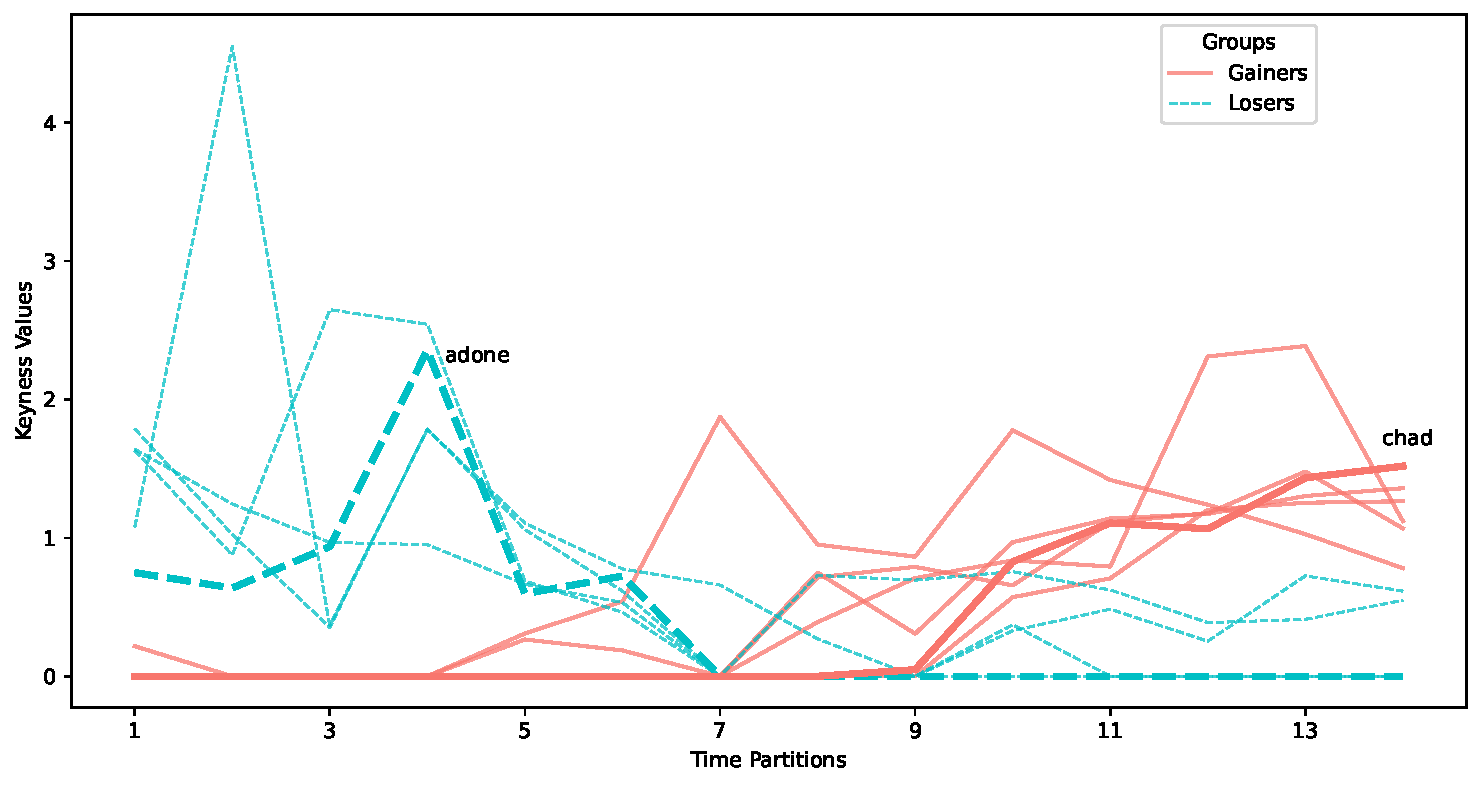
\includegraphics[width=\textwidth]{images-tables/keyness_chart_fdb.pdf}
%     \caption{\itforum}
%   \end{subfigure}
%   \begin{subfigure}[b]{\textwidth}
%     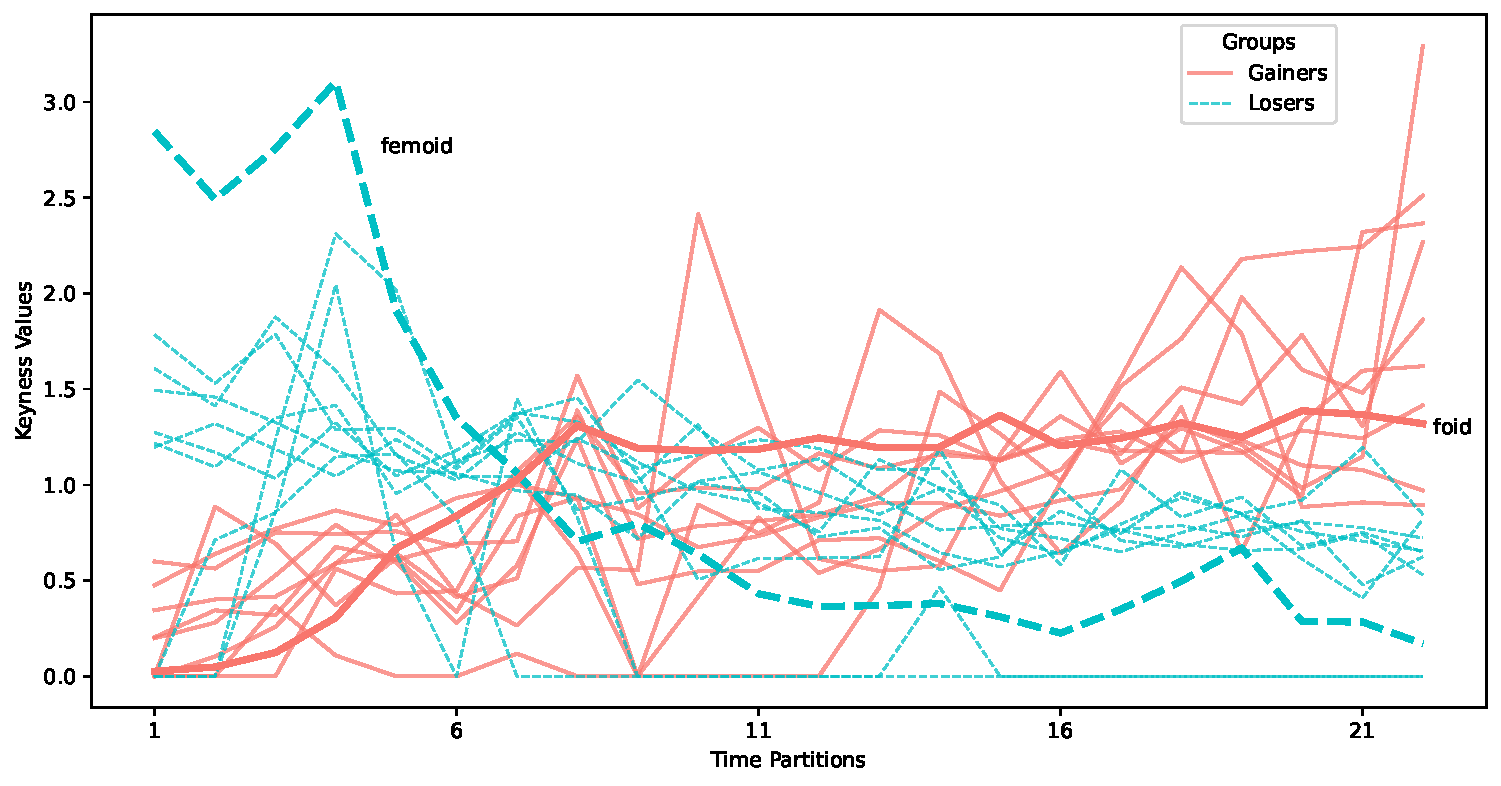
\includegraphics[width=\textwidth]{images-tables/keyness_chart_incelsis.pdf}
%     \caption{\enforum}
%   \end{subfigure}
%   \caption[Keyness graph for \itforum\, and \enforum.]{Keyness over time for the characteristic incel terms extracted from (a) \itforum\, and (b) \enforum. Red lines represent the terms that gained keyness over time, while blue lines represent the terms that lost keyness over time.}
%   \label{fig:keyness-over-time}
% \end{figure*}

% \begin{table}[t]
%   \caption{Keyness normalized slopes for \enforum\, and \itforum.}
%   \footnotesize
%     \centering
%     \begin{tabular}{c|lc|lc}
%       \hline
%       \multirow{2}{*}[0pt]{\rotatebox[origin=c]{0}{\bf Forum}} & \multicolumn{2}{c|}{\bf Gainers} & \multicolumn{2}{c}{\bf Losers} \\
%       \cline{2-5}
%        & \bf Term &\bf  Slope &\bf  Term &\bf  Slope \\
%       \hline
%       \multirow{6}{*}[14pt]{\rotatebox[origin=c]{90}{\begin{minipage}{2cm}\textit{Il forum}\\ \textit{dei brutti}\end{minipage}}}
%       &zerbini & 0.104 & reietto & -0.142 \\
%       &normie & 0.121 & strafigo & -0.122 \\
%       &bv & 0.125 & figaccione & -0.122 \\
%       &chad & 0.126 & attraente & -0.113 \\
%       &subumano & 0.158 & adone & -0.103 \\
%       \cline{2-5}
%       &\bf Mean &\bf 0.127 &\bf Mean &\bf -0.120 \\
%       \hline
%       \multirow{11}{*}[0pt]{\rotatebox[origin=c]{90}{\enforum}} & shitskin    & 0.093           & racepill    & -0.019           \\
%       & deathnic    & 0.081           & stacie      & -0.022           \\
%       &cumskin     & 0.079           & jb          & -0.027           \\
%       &noodlewhore & 0.077           & chadlite    & -0.029           \\
%       &slav        & 0.068           & whitecels   & -0.032           \\
%       &foid        & 0.058           & cunt        & -0.036           \\
%       &curryland   & 0.051           & slut        & -0.046           \\
%       &aryan       & 0.048           & deathnik    & -0.047           \\
%       &ricecel     & 0.047           & roastie     & -0.051           \\
%       &whore       & 0.025           & femoid      & -0.124           \\
%       \cline{2-5}
%       &\bf Mean       &\bf 0.063  &\bf Mean       &\bf -0.043      \\
%       \hline
%     \end{tabular}
%   \label{tab:keyness}
% \end{table}

% Table~\ref{tab:keyness} reports the normalized slopes of the terms obtained from the two forums. In both cases, the mean normalized slopes of the two data series, compared side by side, quantitatively display a clear trend according to which certain terms gain popularity over time, while others become less popular. With regard to \itforum\, the difference is 0.247, while for \enforum\, the difference between the mean normalized slopes is smaller, 0.106, which points at a slower lexical evolution. As regards \enforum, the trends observed for terms such as ``foid'', ``femoid'', and ``roastie'' reflect the time-series data discussed in \newcite{gothard2020exploring}, which show certain terms increasing and decreasing in use over the total messages posted in incel subreddits. For both forums, the shift in lexicon needs to be taken into account in order to have a clear picture of the language adopted by each speech community.

% As regards \itforum, we can observe that the way users refer to men changes in a rather clear way. On one hand, positive words that are commonly used in general language, such as ``strafigo'' and ``figaccione'' (both meaning ``extremely handsome''), are substituted by specialized terms that are more specific to the forum's speech community, e.g., ``chad''.\footnote{\url{https://incels.wiki/w/Chad}} On the other hand, we can see the same phenomenon for negative words, where ``reietto'' (``outcast'') loses popularity, leaving space to terms with more specialized uses, such as ``bv'', meaning ``brutto vero'' (lit. ``truly ugly'') and ``subumano'', meaning ``subhuman''. The first is an acronym, which makes its meaning opaque to outsiders, while the second is a term with a much stronger and denigrating connotation.

% With relation to \enforum, as already anticipated through Figure~\ref{fig:keyness-over-time}, although terms like ``foid'' and ``femoid'' have the same meaning (both are used to dehumanize women by associating them to insentient androids\footnote{\url{https://incels.wiki/w/Femoid}}), the shorter form has become more popular, while the use of the full form has decreased. This is probably due to the fact that, given the high frequency with which the term is used in the forum, users tend to use the abbreviated version to save time and effort. This might seem like a minor detail, but the sheer amount of misogyny that is expressed in the forum through this term alone makes it important to point out a shift in its use.

% % This trend is also confirmed statistically. For both forums, we first take the normalized average slopes for each term and then we test if the difference between gainers and losers of keyness is statistically significant. For the \enforum\, forum, since the data series of the losers is not normally distributed, we use the Mann-Whitney U test \cite{mann1947test}. For \itforum, since both data series are normally distributed, we use a two-sample t-test \cite{snedecor1989statistical}. In both cases, the p-values are well below 0.001, as shown in Table~\ref{tab:statistical-tests-diachronic-study}, showing the results are statistically significant. This means that the change in the usage of the terms is not random, but rather due to a concrete variation in the way specific lexicon is used by the two speech communities.

% % \begin{table}[t]
% %   \centering
% %   \caption[Keyness statistical tests.]{Results of the Mann-Whitney U test and the t-test for the normalized slopes of the keyness of the terms gaining and losing popularity over time, for \enforum\, and \itforum, respectively.}
% %   \label{tab:statistical-tests-diachronic-study}
% %   \begin{tabular}{l|c|c|c}
% %     \hline
% %   \bf Forum                    &\bf  Test       &\bf  Stat Value  &\bf  \textit{p}-Value        \\
% %   \hline
% %   \enforum\,           & Mann-Whitney U & 100             & 0.0002             \\
% %   \itforum\, & t-test         & -22.7566        & 1.4736 x $10^{-8}$ \\
% %   \hline
% %   \end{tabular}
% %   \end{table}

% Based on the conducted qualitative and quantitative analyses, the same conclusions can be drawn for both forums: the presented terms are arguably characteristic of the incel language used within the two platforms and the change in their usage over time is non-negligible. This implies that language models could become progressively worse at predicting over these domains, were their training resources not be periodically updated. Models rely on training material to learn language, and if the material is outdated, their understanding of the discourse currently produced by a specific speech community could become suboptimal.

% Although the hate speech expressed in \itforum\, is not as explicit as in \enforum, having updated resources is still valuable, since they can be used to domain-adapt models to improve their contextual embeddings, for example with Transformer models. Of course, when hate speech is expressed through racist and misogynous neologisms, such as in \enforum, having updated lexical resources becomes of paramount importance.

% In both scenarios, it is thus arguably desirable, if not necessary, to periodically update corpora to have accurate terminological representations. In some cases, it would arguably make sense to even rebuild resources from scratch, were they too outdated. In our case, given the observed changes in keyness, we estimate that the hereby analyzed time frame could be taken as a reference for how long resources can be considered up-to-date. However, with the aim of obtaining an objective figure, further research could be conducted to quantify how often resources should be updated to keep up with the evolution of the language used in the spaces scrutinized through this study.

% The necessity to build such material is also supported by the fact that resources on the topic of incels are rare and limited, and their applicability is often compromised because the linguistic domain of the source data only partially aligns with the one under investigation~\cite{pelzer-2021-toxic-language-incel-communities}. An additional cause for such incompatibility of resources can be found in the annotation scheme, which can be inapplicable to the supervised task being approached~\cite{zhou-2022-automated-hs-detection}. However, the necessity to build new resources does not mean they will be obsolete soon after being employed, as the time frames we have analyzed in this chapter span various years of forum activity.

\end{document}
